\flushleft
\textbf{Theoretical Framework}\\

\begin{figure}[H]
	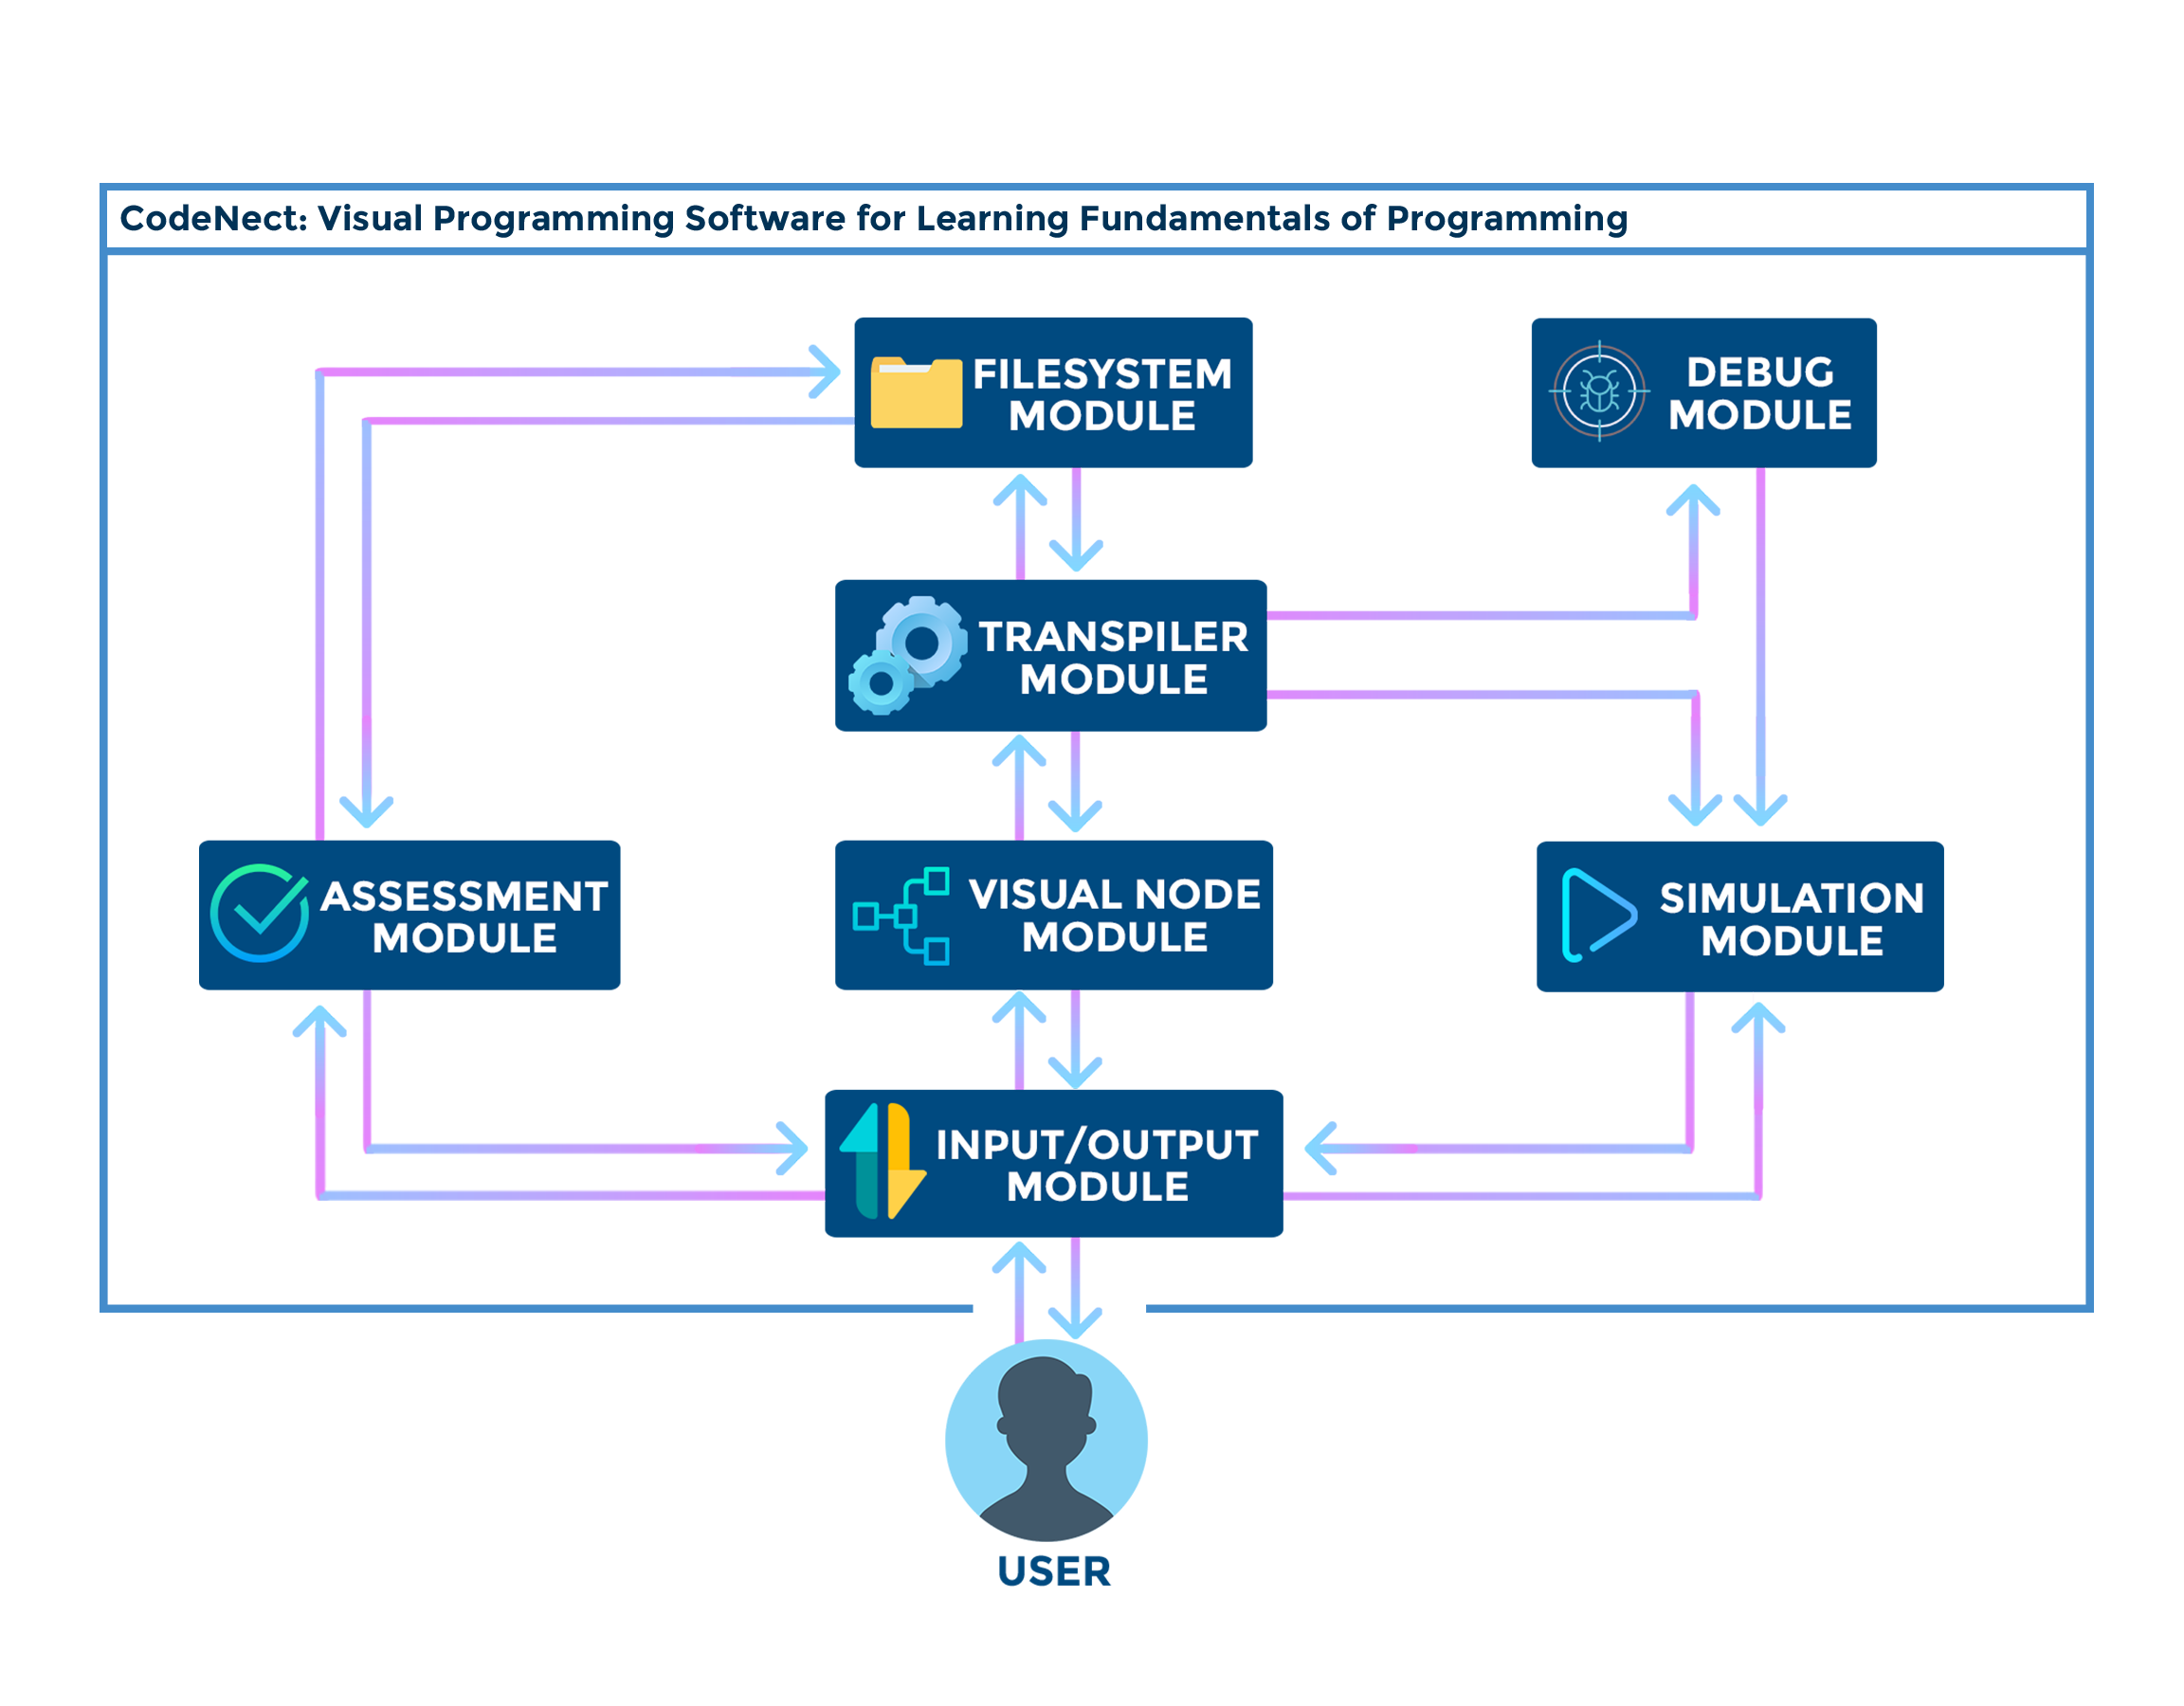
\includegraphics[width=\linewidth]{figures/theoretical_framework.png}
	\caption{Theoretical Framework of proposed Visual Programming Software for Learning
	Fundamentals of Programming}
	\label{fig:theoretical_framework}
\end{figure}

\justifying
The graphical representation of the modules and its inter-relation and inter-dependency
provides an overview of the process for the theoretical framework proposed. The core
features of each module function as solutions to the identified problems.

\par
The framework is closely designed to adhere to the study of Six Learning Barriers in
End-User Programming Systems (\cite{ko_myers_aung_2004}) wherein each module is designed
to reduce the occurence of other barriers (\cite{dao_bøg_2010}). The Design barrier is
alleviated through the implementation of visual programming instead of the traditional
text-based programming. The Selection barrier is aided through the basic data types and
structures constraints. The Coordination barrier is eased through the visually
observing nodes, graphs, and wires elements. The Use barrier is lightened to the basic
and necessary tools only available and provided. The Understanding barrier is solved by
observing the simulation. And the Information barrier is minimized by the interactive
debugging and simulation features.

\par
The \textbf{User} can be a student, instructor, or anyone who uses the software. The
user is responsible for the implementation, organization, testing, and experimentation
of the elements responsible for the code logic in represented via visual nodes and
graph. The user also decides for project creation, modification, and deletion as well
as running and debugging the code. The user can also opt to go to the assessment mode.

\par
The \textbf{Input and Output Module} handles the input events emitted from the interaction
of the user with the software either through the keyboard or the mouse. Events such as
key press, key release, mouse left click, mouse right click, and mouse wheel scroll are
handled accordingly to the context within the software if whether the event occured
within the view of the visual programming interface, in simulation, or in assessment.

\par
For richer user experience, the module also returns feedback for the user in
response to the input. This is handled by the output sub-module which also manages
the visual interface such as the views and elements which the user sees. The sub-module
handles the state of the software whether in visual programming interface, in simulation,
or in assessment.

\par
The \textbf{Filesystem Module} processes the projects stored. Upon the launch of the
software, the directory where projects are stored are read for validation as well as
fetching of internal data for the list of recent projects. When user opens a project,
the selected project and all its files are fetched, loaded, and displayed to the user.
The module also acts as the interface between the user and the operating system for
managing resources and file permissions to assure that no unsafe commands are executed
that may tamper the software, the files, or even the system of the user. During
simulation, files that are transpiled and temporary are stored and cached for efficiency
and less build time.

\par
The \textbf{Visual Nodes Module} presents the graphical elements to the screen that are
necessary for building and coding logic. This module is interacted by the user through
the Input and Output Module where mouse clicking in a node opens a context and dragging
it moves the node. The Visual Nodes Module also renders the views through a camera.
This is useful for panning and zooming across the whole screen without having to move
the nodes and graphs along.

\par
This module technically are just sets of data and logic. It does not handle the actual
rendering of the components. The Output sub-module handles the drawing by referencing
the data stored in the Visual Nodes Module. This approach is flexible and extensible as
it can easily adapt and be used with other renderers other than the provided one.

\par
The \textbf{Transpiler Module} is an internal module that is abstracted to the user and
acts as the middleware between the Visual Nodes Module and the Simulation Module. The
module compiles and builds the visual code as input by the user and the Simulation
Module handles running the transpiled source code.  This module is also extensible so
that more target programming languages can be added by contributors or the community if
desired. This module also checks for file changes, if there is none, instead of
repeating the same process that will yield to the same results, it will fetch the
cached files through the Filesystem module and use that instead for instant process.

\par
The \textbf{Simulation Module} runs after the transpilation stage. After a successful
compilation and building of the visual code to the target programming language, the
source code is run and simulated for the user to see the result of the code. Depending
on the visual code made by the user, the simulation can also accept input from the user
as a normal and typical program that runs in the terminal.

\par
The \textbf{Debug Module} runs concurrently with the Transpilation and Simulation Modules.
An error or warning during the transpilation stage will notify the user with detailed
information, possible cause, explanation, and help in fixing it. If there is a runtime
error or exception during the simulation stage, the Debug Module will handle it and
provide a cleaner and beginner-friendly message.

\par
The \textbf{Assessment Module} is a module that handles operations during the assessment
mode. This mode fetches files through the Filesystem Module and serves a list of possible
questions and exercises oriented towards learning fundamentals of programming. Upon the
selection of user, this module handles input and output of the user and performs
evaluation to the visual code as the answer or solution of the user. The results are
presented to the user and stored in the filesystem as well. This module has the function
of providing report about the activity and assessment of the user.\\
